\documentclass[12pt, a4paper]{article}

% Text languages
\usepackage[english, UKenglish, USenglish, american, british]{babel}

% Accents
%usepackage[latin1]{inputenc}

% Maths
\usepackage{mathtools}
\usepackage{amsmath,amsthm,amssymb}

% Double rows
%\usepackage{multirow}

% Math-mode symbol & verbatim
%\def\W#1#2{$#1{#2}$ &\tt\string#1\string{#2\string}}
%\def\X#1{$#1$ &\tt\string#1}
%\def\Y#1{$\big#1$ &\tt\string#1}
%\def\Z#1{\tt\string#1}

% A non-floating table environment.
%\makeatletter
%\renewenvironment{table}%
%   {\vskip\intextsep\parskip\z@
%    \vbox\bgroup\centering\def\@captype{table}}%
%   {\egroup\vskip\intextsep}
%\makeatother

%\DeclarePairedDelimiter\abs{\lvert}{\rvert}%
%\DeclarePairedDelimiter\norm{\lVert}{\rVert}%

% Swap the definition of \abs* and \norm*, so that \abs
% and \norm resizes the size of the brackets, and the 
% starred version does not.
%\makeatletter
%\let\oldabs\abs
%\def\abs{\@ifstar{\oldabs}{\oldabs*}}
%
%\let\oldnorm\norm
%\def\norm{\@ifstar{\oldnorm}{\oldnorm*}}
%\makeatother

% C++
\usepackage{listings}
\usepackage{xcolor}
\lstset { %
	language = C++,
	backgroundcolor=\color{black!5}, % set backgroundcolor
    basicstyle=\footnotesize,% basic font setting
    tabsize=4, % tab space width
    showstringspaces=false, % don't mark spaces in strings
    %numbers=left, % display line numbers on the left
    commentstyle=\color{green}, % comment color
    keywordstyle=\color{blue}, % keyword color
    stringstyle=\color{red} % string color
}

% https://www.overleaf.com/learn/latex/Page_size_and_margins
\usepackage{geometry}
\topmargin = -23pt
\oddsidemargin = 13pt
\headheight = 12pt
\headsep = 25pt
\textheight = 674pt
\textwidth = 426pt
\marginparsep = 10pt
\marginparwidth = 50pt
\footskip = 30pt
\marginparpush = 5pt
\hoffset = 0pt
\voffset = 0pt
\paperwidth = 597pt
\paperheight = 845pt

% Hyperlinks
\usepackage{hyperref}

% Figure
\usepackage{graphicx}
\usepackage{caption}
\usepackage{subcaption}
\usepackage{etoc}
% Example
\newtheorem{exmp}{Example}[section]
% Algorithms
%\usepackage[]{algorithm2e}
%\usepackage{algorithm}% http://ctan.org/pkg/algorithm
%\usepackage{algpseudocode}% http://ctan.org/pkg/algorithmicx
\usepackage{algpseudocode}

\renewcommand{\thefootnote}{\arabic{footnote}} % 1, 2, 3... (la que hay por defecto)

\setcounter{secnumdepth}{5}
\setcounter{tocdepth}{5}

%\titleformat{\paragraph}
%{\normalfont\normalsize\bfseries}{\theparagraph}{1em}{}
%\titlespacing*{\paragraph}
%{0pt}{3.25ex plus 1ex minus .2ex}{1.5ex plus .2ex}

\usepackage{float}
%--------------------------------------------------------------------------
\title{PARALLELISM}
\author{Roger Vilaseca Darné and Xavier Martín Ballesteros\\
  \small UNIVERSITAT POLITÈCNICA DE CATALUNYA\\
}
\date{10th December 2018}

\begin{document}
% Images
\graphicspath{ {./images} }

%\maketitle

\begin{titlepage}
	\centering
%	{\scshape\LARGE UNIVERSITAT POLITÈCNICA DE CATALUNYA \par}
	\vspace{1cm}
	{\scshape\Large UNIVERSITAT POLITECNICA DE CATALUNYA\par}
	\vspace{1.5cm}
	{\huge\bfseries PARALLELISM\par}
	\vspace{2cm}
	{\Large\itshape \textbf{Lab 4: Divide and Conquer parallelism with OpenMP: Sorting}\par}
	\vfill
	{\Large\itshape Roger Vilaseca Darne and Xavier Martin Ballesteros\break PAR4110\par}
	\vfill
	
\includegraphics[width=0.25\textwidth]{./images/UPC.png}\par\vspace{1cm}
	%supervised by\par
	%Dr.~Mark \textsc{Brown}

	\vfill

% Bottom of the page
	{\large 15th May 2019, Q2}
\end{titlepage}

%\abstract{Esto es una plantilla simple para un articulo en \LaTeX.}

%	*********************** ÍNDEX *********************
\setcounter{secnumdepth}{5}

\newpage
  \tableofcontents
\newpage

% Referència a una equació \ref{eq:area}).
% Referència a una secció \ref{sec:nada}
% Referència a una cita \cite{Cd94}.

\section{Introduction}

\section{Anlysis with \textit{Tareador}}

In order to study which is the best approach that we should use to parallelize the code (using the \textit{OpenMP} directives), a study about the task dependencies is needed.

In the following subsections, we will analyse the functions \textit{merge} and \textit{multisort} of the given code using \textit{Tareador} to see the potential parallelism they have and also their dependences. As both functions are recursive, it is very likely that we will be able to parallelise them.

The modified code can be found in the \textit{multisort-tareador.c} file, inside the codes directory.

\subsection{Merge Function}

The merge function is responsible for sorting two vectors, merging them into one. This is done using recursive calls that divide the vectors into smaller ones.

Our study in this function focuses on the two recursive calls done in the else fragment of the function. A task is created every time we make a recursive call to the function. As a consequence, some created tasks will also execute the basicmerge function.

To do that, we have used the \textit{tareador\_start\_task} and \textit{tareador\_end\_task} functions. The resulting code is shown below.

\begin{figure}[H]
\begin{lstlisting}
void merge(long n, T left[n], T right[n], T result[n*2], long start,
		   long length) {
    if (length < MIN_MERGE_SIZE*2L) {
        // Base case
        basicmerge(n, left, right, result, start, length);
    } else {
        // Recursive decomposition
        tareador_start_task("me1");
        merge(n, left, right, result, start, length/2);
        tareador_end_task("me1");

        tareador_start_task("me2");
        merge(n, left, right, result, start + length/2, length/2);
        tareador_end_task("me2");
    }
}
\end{lstlisting}

\label{code:merge_tareador}
\caption{Modified version of the merge function.}
\end{figure}


\subsection{Multisort Function}

The multisort function divides the input vector into 4 smaller vectors, apply a recursive call for each of them and then merges the 4 vectors into a big sorted one.

We will use the same strategy than in the merge function. This is, creating a task for each recursive call and for each call to the merge function.

We have also used the \textit{tareador\_start\_task} and \textit{tareador\_end\_task} functions. The code is the following:

\begin{figure}[H]
\begin{lstlisting}
void multisort(long n, T data[n], T tmp[n]) {
    if (n >= MIN_SORT_SIZE*4L) {
        // Recursive decomposition
        tareador_start_task("mu1");
        multisort(n/4L, &data[0], &tmp[0]);
        tareador_end_task("mu1");

        tareador_start_task("mu2");
        multisort(n/4L, &data[n/4L], &tmp[n/4L]);
        tareador_end_task("mu2");

        tareador_start_task("mu3");
        multisort(n/4L, &data[n/2L], &tmp[n/2L]);
        tareador_end_task("mu3");

        tareador_start_task("mu4");
        multisort(n/4L, &data[3L*n/4L], &tmp[3L*n/4L]);
        tareador_end_task("mu4");

        tareador_start_task("me1");
        merge(n/4L, &data[0], &data[n/4L], &tmp[0], 0, n/2L);
        tareador_end_task("me1");

        tareador_start_task("me2");
        merge(n/4L, &data[n/2L], &data[3L*n/4L], &tmp[n/2L], 0, n/2L);
        tareador_end_task("me2");


        tareador_start_task("me3");
        merge(n/2L, &tmp[0], &tmp[n/2L], &data[0], 0, n);
        tareador_end_task("me3");

    } else {
        // Base case
        basicsort(n, data);
    }
}
\end{lstlisting}

\label{code:multisort_tareador}
\caption{Modified version of the multisort function.}
\end{figure}

\subsection{Task dependency graph (TDG)}
\label{subsec:TDG}

We can clearly see that Figure \ref{fig:TDG} is divided into two parts: the multisort and the merge.

As we said before, in the multisort function we divide the input vector into 4 smaller vectors, until the vector size is smaller than $MIN\_SORT\_SIZE \times 4L$. This can be seen at the top of the figure, as we can see 4 different boxes (green, red, yellow and purple). Moreover, there is no data sharing between them, so we can execute them at the same time.

Then, there is a new recursion level inside each box. These four calls reach the limit value, so they do a \textit{basicmerge} call. Afterwards, we need the first two childs to terminate before executing the first merge call (and the same for the third and fourth childs with the second merge call). Thus, there exist a dependence between the recursive calls to multisort and the calls to the first two merge functions. Finally, the third merge call can be executed only when the previous two merge calls have terminated (another dependence).

On the other hand, in the merge function, we create tasks when the number of elements of the vector that we want to sort is bigger or equal than $MIN\_MERGE\_SIZE \times 2L$. We see in the figure that the two created tasks do not have any dependence between them. A \textit{basicmerge} call will be done when we reach the limit value.

\begin{figure}[H]
	\centering
	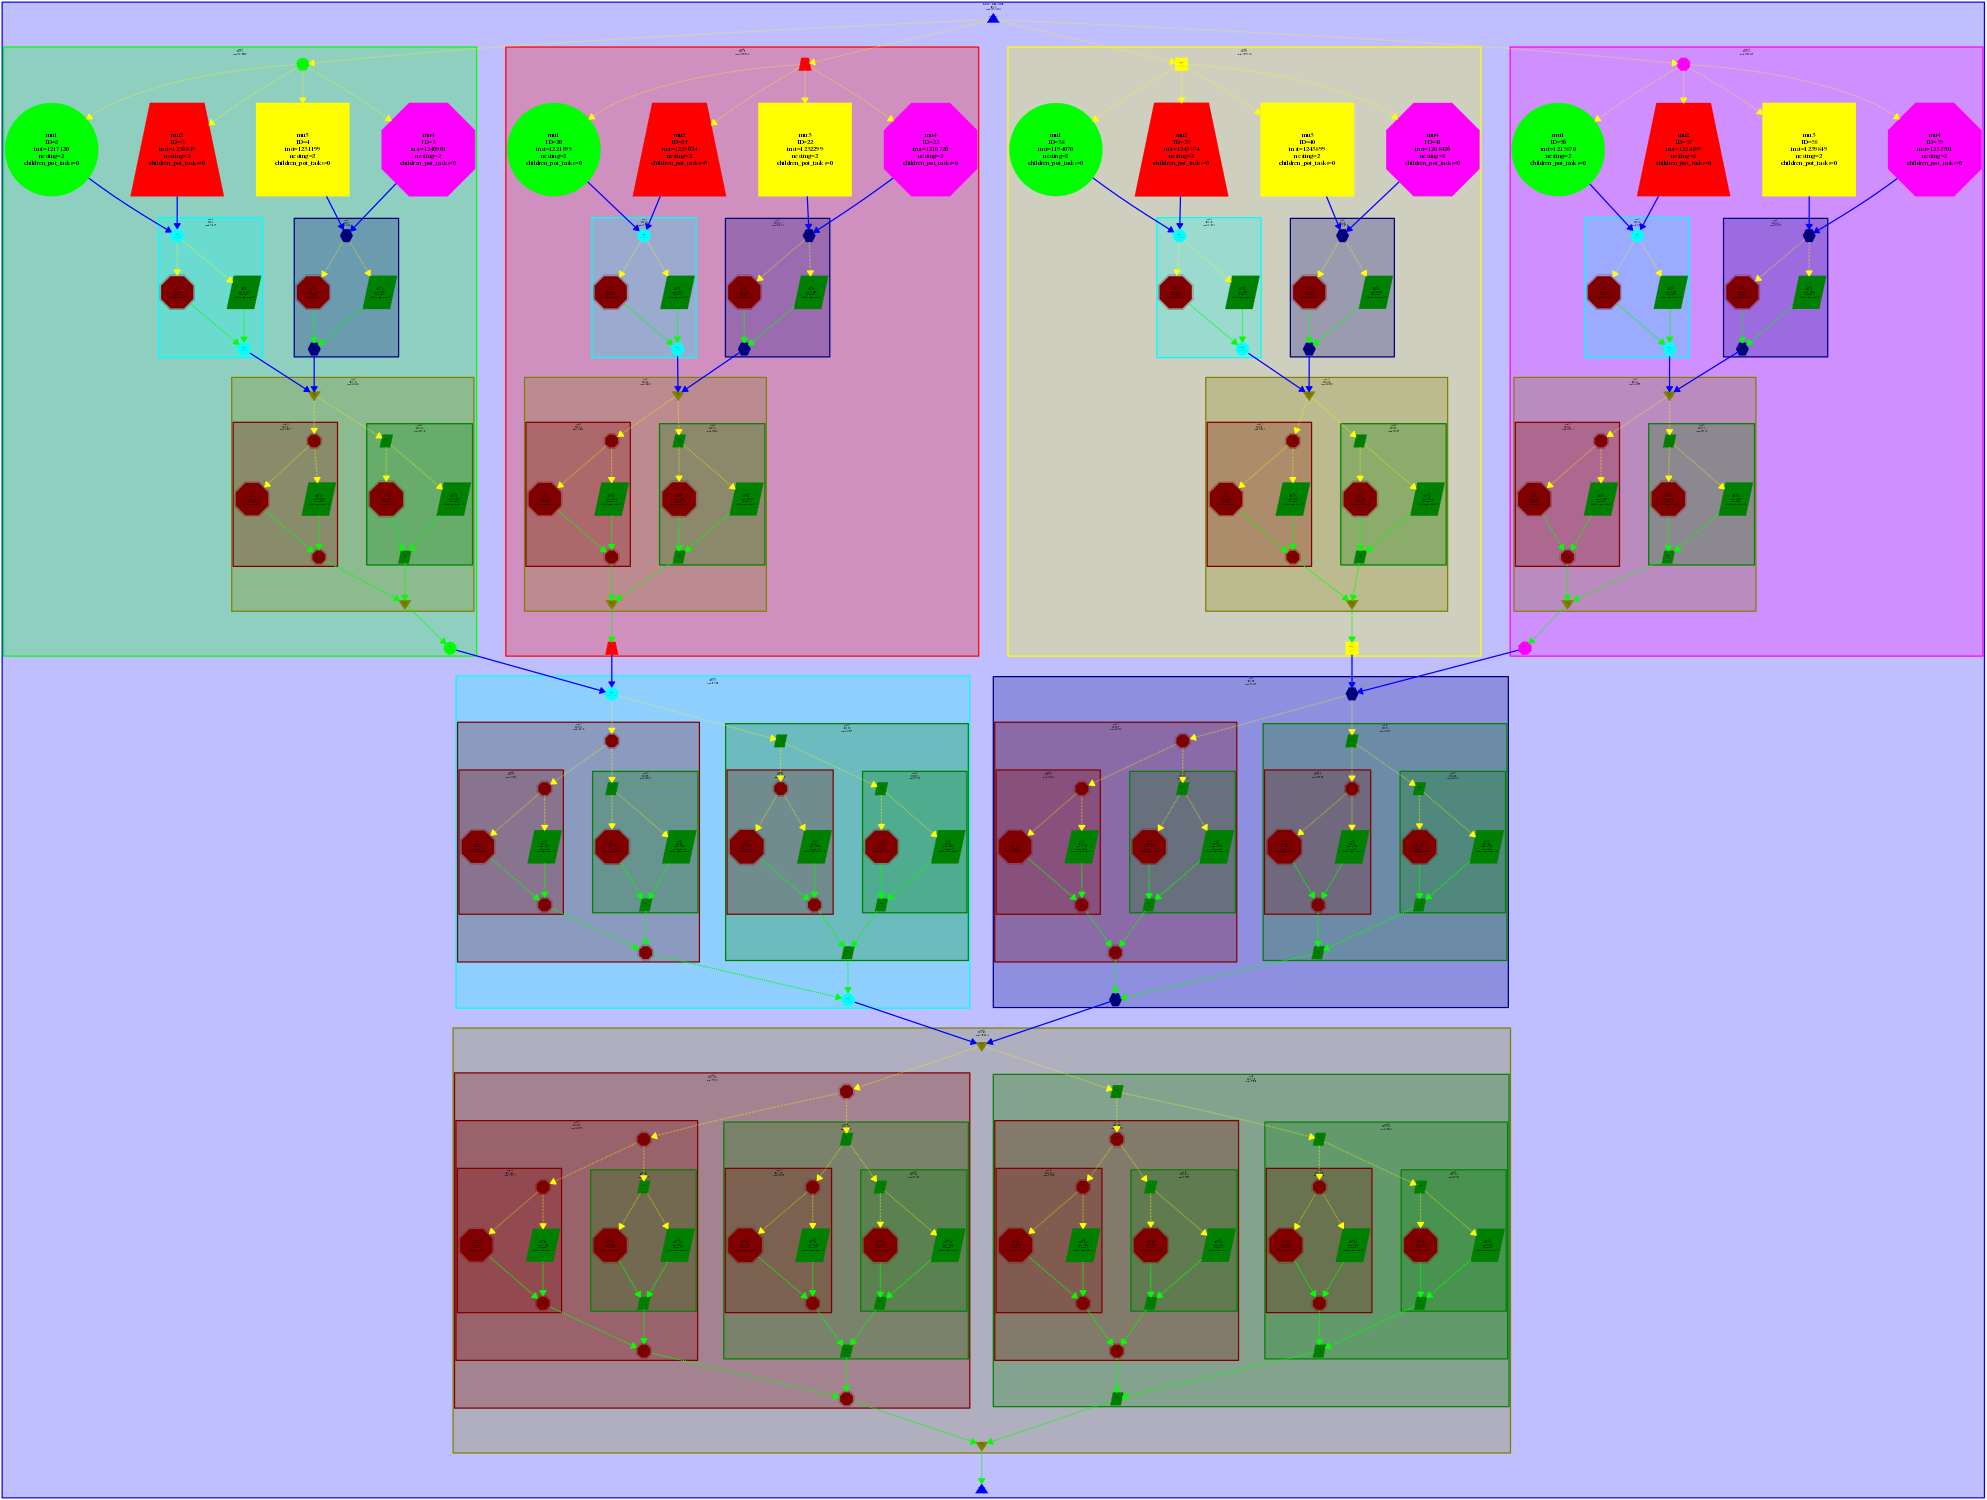
\includegraphics[scale=0.16]{./images/dependency_graph}
	
	\label{fig:TDG}
	\caption{Task dependency graph obtained using \textit{Tareador}.}
\end{figure}

With all these information, we can conclude that we can use a \textbf{Tree strategy} (generate a task for each recursive function) because there are no dependences between sibling tasks. Besides, we can also use a \textbf{Leaf strategy} (generate a task in each base case of the functions).

Furthermore, we must be careful about the synchronization we need between the multisort tasks and the merge ones because, as we said before, the first merge call depends on the first two multisort calls, the second merge call depends on the third and fourth multisort calls and the third merge call depends on the previous two merge calls. Without synchronization we would have wrong results due to data racing.

\subsection{Parallel Performance and Scalability}

The following table shows the execution time and speed-up values obtained when varying the number of processors.

\begin{table}[H]
\centering
\begin{tabular}{ |c|c|c| } 
 \hline
 \textbf{Processors} & \textbf{Execution Time [ns]} & \textbf{Speed-Up} \\ 
 \hline
 \hline
	1	& 20334411001	& 1 \\
	 \hline
	2	& 10173716001	& 1.99872013323365 \\
	 \hline
	4	& 5086725001	& 3.99754478510288 \\
	 \hline
	8	& 2550595001	& 7.97241858979085 \\
	 \hline
	16	& 1289922001	& 15.7640624667507 \\
	 \hline
	32	& 1289909001	& 15.7642213406029 \\
	 \hline
	64	& 1289909001	& 15.7642213406029 \\
 \hline
\end{tabular}
 
 \label{tab:Scalability_S1}
\caption{Execution Time and Speed-Up varying the number of processors.}
\end{table}

We can see that until 16 processors, the results obtained are pretty close to the ideal ones. However, from 16 to infinite processors there is no improvement on the speed-up values. This is because in Figure \ref{fig:TDG} we see that the maximum number of tasks executed at the same time are 16. For this reason, using more than 16 processors will not have any impact on the execution time and speed-up.

\begin{figure}[H]
\hspace{-0.5cm}
\begin{subfigure}{.5\textwidth}
  \centering
  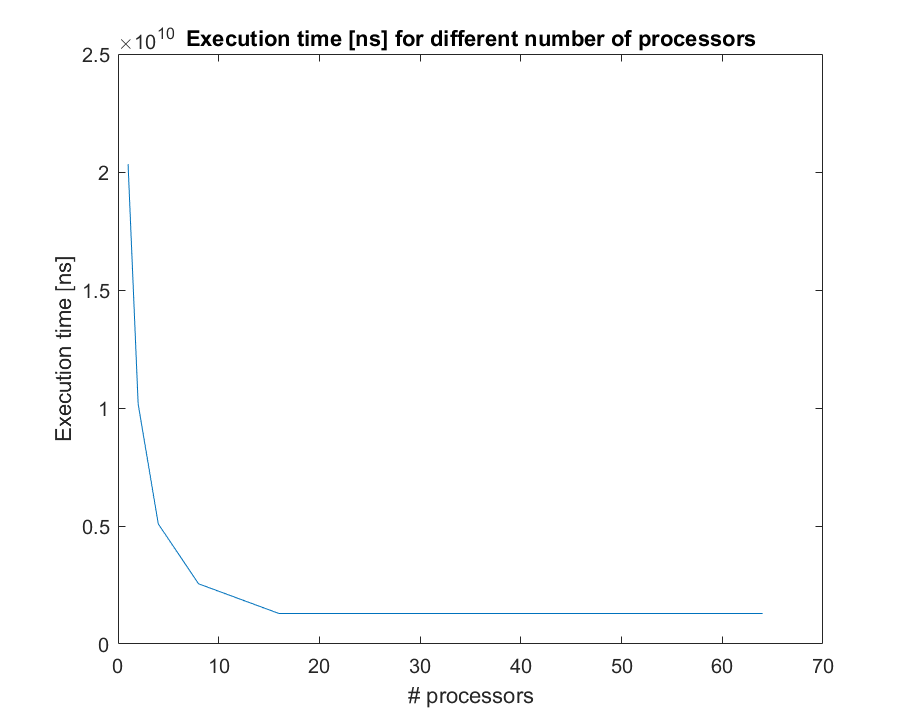
\includegraphics[width=1.10\linewidth]{./images/S1_plots/execution_time_line}
  
\end{subfigure}%
\begin{subfigure}{.5\textwidth}
  \centering
  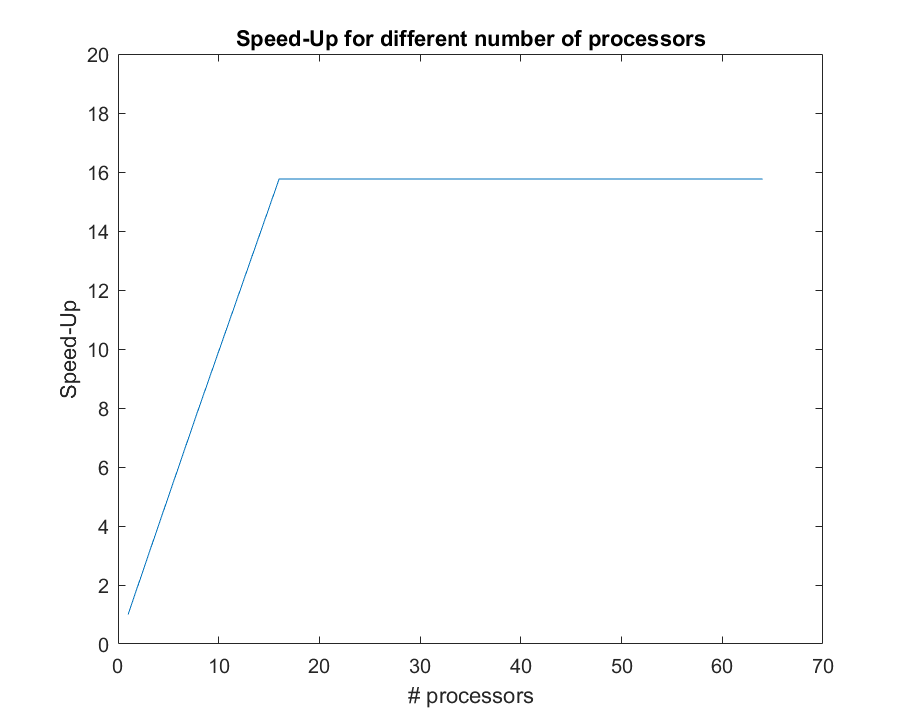
\includegraphics[width=1.10\linewidth]{./images/S1_plots/speedup_line}

\end{subfigure}
\caption{Execution Time and Speed-Up plots varying the number of processors.}
\end{figure}

\break

\textbf{Include the relevant parts of the modified multisort-tareador.c code and comment where the
calls to the Tareador API have been placed. Comment also about the task graph generated and
the causes of the dependences that appear.}

\textbf{Write a table with the execution time and speed-up predicted by Tareador (for 1, 2, 4, 8, 16, 32
and 64 processors) for the task decomposition specified with Tareador. Are the results close to the
ideal case? Reason about your answer.}

\section{Parallelization and performance analysis with tasks}

As we said in the previous section, we concluded that we can use both Tree and Leaf strategies for the parallelization of the multisort and merge functions.

In this section we are going to analyse the parallelization and performance of the 2 strategies implemented using the \textit{OpenMP} clauses. The different versions of the code can be found in the next subsections. Nevertheless, the following code will be the same for the implementation of both strategies:

\begin{figure}[H]
\begin{lstlisting}
#pragma omp parallel
#pragma omp single
multisort(N, data, tmp);
\end{lstlisting}

\caption{Modified fragment of the given code in the main function.}
\end{figure}

\subsection{Leaf Strategy}

In this strategy, we define a task for the invocations of basicsort and basicmerge functions. That is, we create a task each time we are in the base case of multisort and merge functions.

In order to do it, we have used the \textit{\#pragma omp task} clause. As we have seen in the section \ref{subsec:TDG}, there exists dependencies between some function calls, so we will need an \textit{OpenMP} clause to synchronize these functions (\textit{\#pragma omp taskwait}).

The code can be found in the \textit{multisort-omp-leaf.c} file inside the codes directory. However, the important changes of the code are shown below.

\begin{figure}[H]
\begin{lstlisting}
void merge(long n, T left[n], T right[n], T result[n*2], long start,
		   long length) {
    if (length < MIN_MERGE_SIZE*2L) {
        // Base case
        #pragma omp task
        basicmerge(n, left, right, result, start, length);
    } else {
        // Recursive decomposition
        merge(n, left, right, result, start, length/2);
        merge(n, left, right, result, start + length/2, length/2);
    }
}
\end{lstlisting}

\caption{Merge function implementing the Leaf strategy.}
\end{figure}

\begin{figure}[H]
\begin{lstlisting}
void multisort(long n, T data[n], T tmp[n]) {
    if (n >= MIN_SORT_SIZE*4L) {
        // Recursive decomposition
		multisort(n/4L, &data[0], &tmp[0]);
		multisort(n/4L, &data[n/4L], &tmp[n/4L]);
		multisort(n/4L, &data[n/2L], &tmp[n/2L]);
		multisort(n/4L, &data[3L*n/4L], &tmp[3L*n/4L]);
		
		#pragma omp taskwait
		
		merge(n/4L, &data[0], &data[n/4L], &tmp[0], 0, n/2L);
		merge(n/4L, &data[n/2L], &data[3L*n/4L], &tmp[n/2L], 0, n/2L);
		
		#pragma omp taskwait
		
        merge(n/2L, &tmp[0], &tmp[n/2L], &data[0], 0, n);
	} else {
		// Base case
		#pragma omp task
		basicsort(n, data);
	}
}
\end{lstlisting}

\caption{Multisort function implementing the Leaf strategy.}
\end{figure}

We can see in Figure \ref{fig:leaf_traces} that only thread 0 is the one that creates tasks (in the base case of the functions), while the other tasks are executing them. Moreover, we can see that thread 0 is also executing tasks. We think that this happens because it does not create tasks very usually, so it has time to execute some of the tasks inside the pool.

On the other hand, we can also see the effect of the \textit{\#pragma omp taskwait} clause if we look at the first trace of the figure. There are plenty of red parts (synchronization parts) in all threads.

\begin{figure}[H]
	\centering
	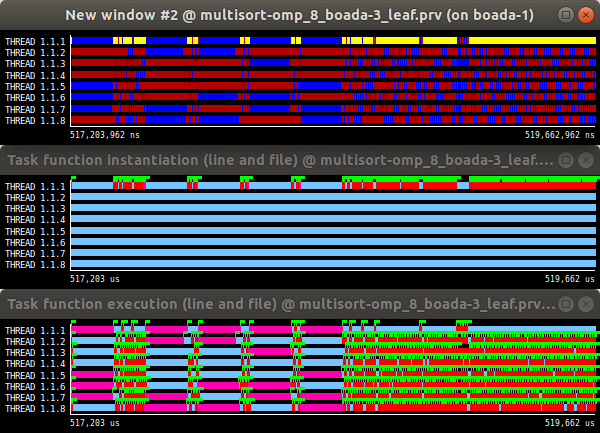
\includegraphics[scale=0.45]{./images/S2/Leaf_paraver}
	
	\label{fig:leaf_traces}
	\caption{Fragment of the execution flow of the code using the Leaf strategy.}
\end{figure}

As in the Leaf stratgy only one thread executes the recursive part of the functions, there is a big amount of time where the other threads are doing nothing. Consequently, the speed-up plots for the complete application and only the multisort function cannot be good.

\begin{figure}[H]
\centering
\begin{minipage}[b]{0.4\linewidth}
  \centering
  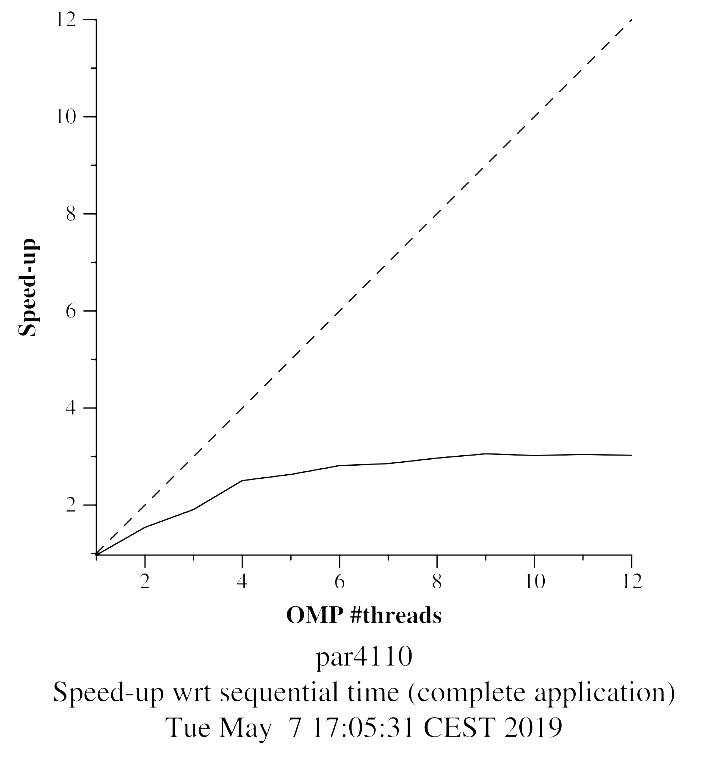
\includegraphics[scale=0.5]{./S2/S2_strong_scalability/multisort-omp-strong_boada-2_leaf_complete_application}
  \caption{Speed-up plot of the complete application using the Leaf strategy.}
  \label{fig:mandel-omp-10000-strong-21-time}
\end{minipage}%
\hspace{0.5cm}
\begin{minipage}[b]{0.4\linewidth}
  \centering
  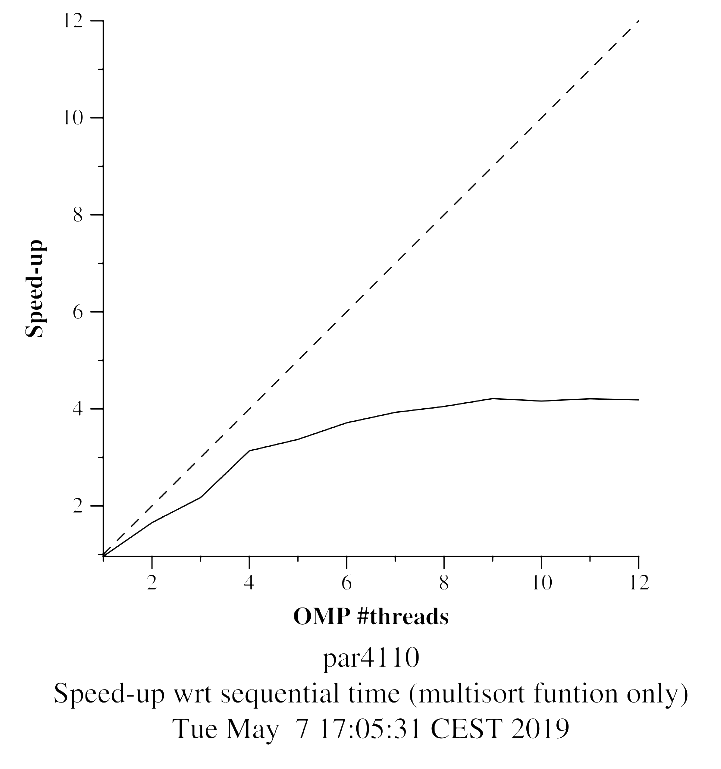
\includegraphics[scale=0.5]{./S2/S2_strong_scalability/multisort-omp-strong_boada-2_leaf_multisort_only}
  \caption{Speed-up plot of the multisort function using the Leaf strategy.}
  \label{fig:mandel-omp-10000-strong-21-speedup}
\end{minipage}
\end{figure}

If we continue adding more threads to execute the code, this will result into an irrelevant improvement of both speed-up plots because there will be more threads that are doing no work, which means that the total amount of time in the Idle state will increase.

\subsection{Tree Strategy}
\label{treestrategy}

In this other strategy, we define a task during the recursive decomposition, when invoking multisort and merge recursive calls.

To do it, we have also used the \textit{\#pragma omp task} clause. However, we cannot use \textit{\#pragma omp taskwait} in the multisort function anymore because we have to stop the flow of the code until a group of recursive calls which some are siblings and others are not terminate. To achieve this, we have used the \textit{\#pragma omp taskgroup} clause. We have done 3 groups taking into account the dependences in Figure \ref{fig:TDG}: multisort calls, first two merge calls and the third merge call.

The following code can be found in the \textit{multisort-omp-tree.c} file inside the codes directory.

\begin{figure}[H]
\begin{lstlisting}
void merge(long n, T left[n], T right[n], T result[n*2], long start,
	 	   long length) {
    if (length < MIN_MERGE_SIZE*2L) {
        // Base case
        basicmerge(n, left, right, result, start, length);
    } else {
        // Recursive decomposition
        #pragma omp task
        merge(n, left, right, result, start, length/2);
        
        #pragma omp task
        merge(n, left, right, result, start + length/2, length/2);
    }
}
\end{lstlisting}

\caption{Merge function implementing the Tree strategy.}
\end{figure}

\begin{figure}[H]
\begin{lstlisting}
void multisort(long n, T data[n], T tmp[n]) {
    if (n >= MIN_SORT_SIZE*4L) {
	    // Recursive decomposition
	    #pragma omp taskgroup
	    {
			#pragma omp task
			multisort(n/4L, &data[0], &tmp[0]);
			
			#pragma omp task
			multisort(n/4L, &data[n/4L], &tmp[n/4L]);
			
			#pragma omp task
			multisort(n/4L, &data[n/2L], &tmp[n/2L]);
			
			#pragma omp task
			multisort(n/4L, &data[3L*n/4L], &tmp[3L*n/4L]);
		}
	
		#pragma omp taskgroup
		{
			#pragma omp task
			merge(n/4L, &data[0], &data[n/4L], &tmp[0], 0, n/2L);
			
			#pragma omp task
			merge(n/4L, &data[n/2L], &data[3L*n/4L], &tmp[n/2L],
				  0, n/2L);
		}
		
		#pragma omp task
	    merge(n/2L, &tmp[0], &tmp[n/2L], &data[0], 0, n);
	} else {
		// Base case
		basicsort(n, data);
	}
}
\end{lstlisting}

\caption{Multisort function implementing the Tree strategy.}
\end{figure}

Now, with this new strategy, all threads can execute and create tasks. At he beginning only thread 0 could create tasks, but each time it creates one, the number of threads that can create tasks increases. As a consequence, the execution time will be reduced a lot because now the total amount of time in the Idle state is reduced.

\begin{figure}[H]
	\centering
	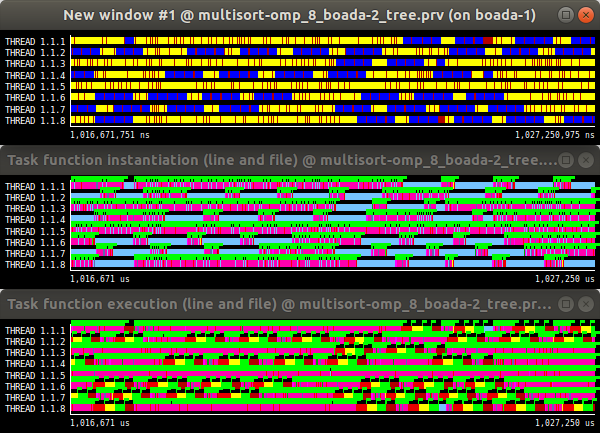
\includegraphics[scale=0.45]{./images/S2/Tree_paraver}
	
	\label{fig:tree_traces}
	\caption{Fragment of the execution flow of the code using the Tree strategy.}
\end{figure}

As we have said before, the execution time is reduced a lot, improving the speed-up plots of both complete application and multisort function only. Hence, both plots will be much better than the ones obtained using the Leaf strategy.

Besides, we can see that this improvement has had a much impact on the multisort function only plot than in the complete application one.

\begin{figure}[H]
\centering
\begin{minipage}[b]{0.4\linewidth}
  \centering
  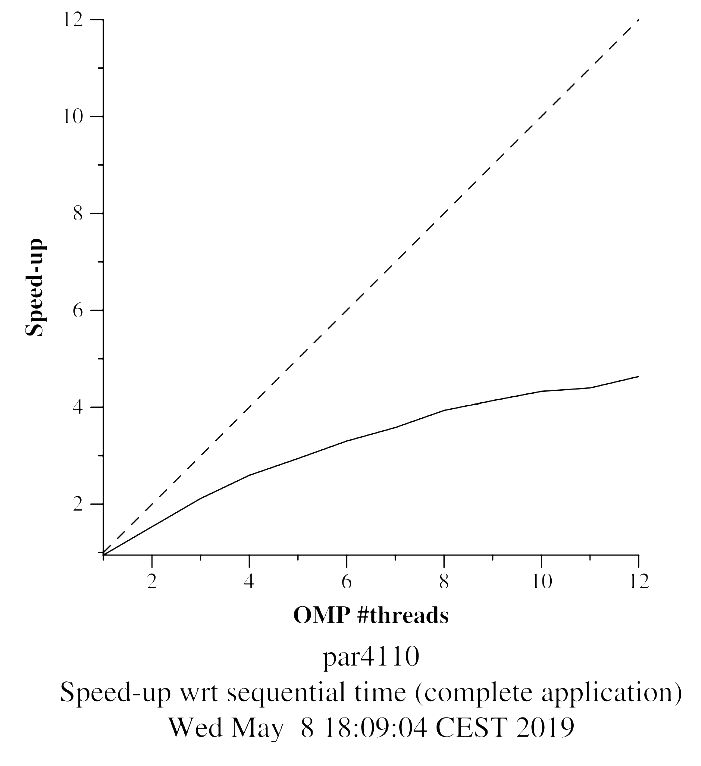
\includegraphics[scale=0.5]{./S2/S2_strong_scalability/multisort-omp-strong_boada-3_tree_complete_application}
  \caption{Speed-up plot of the complete application using the Tree strategy.}
  \label{fig:mandel-omp-10000-strong-21-time}
\end{minipage}%
\hspace{0.5cm}
\begin{minipage}[b]{0.4\linewidth}
  \centering
  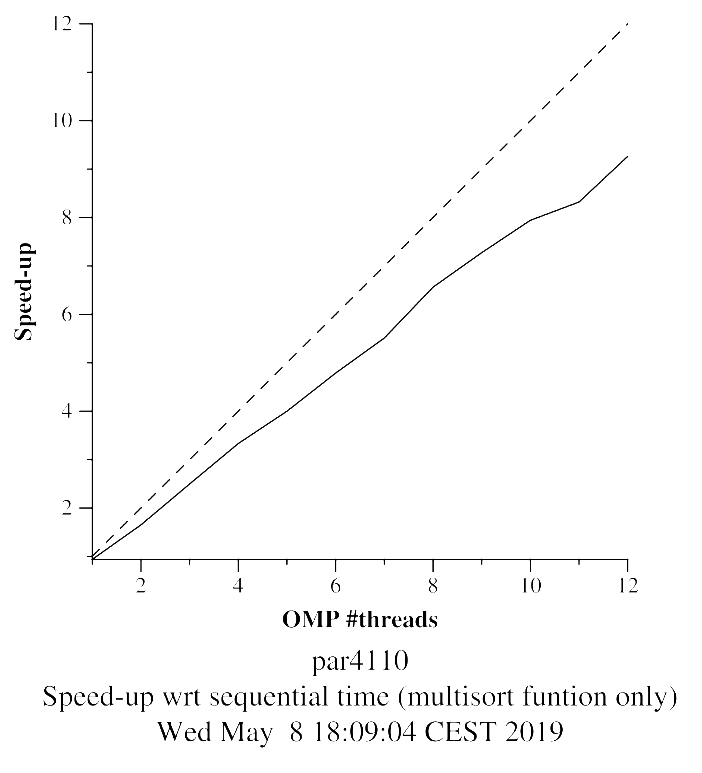
\includegraphics[scale=0.5]{./S2/S2_strong_scalability/multisort-omp-strong_boada-3_tree_multisort_only}
  \caption{Speed-up plot of the multisort function using the Tree strategy.}
  \label{fig:mandel-omp-10000-strong-21-speedup}
\end{minipage}
\end{figure}

If we continue adding more threads to execute the code, this will result into a better performance of the code. We would have better execution time and speed-up results.

\subsection{Task Cut–Off Mechanism}

As we have seen, in the Tree strategy there is not a maximum recursion level, so if we have a large vector input we can be calling functions recursively for a long time.

To solve this problem, we can set a maximum recursion level using a cut-off mechanism that controls it for task generation (and their granularity).

To do this, we have used the \textit{final(condition)} clause. When the condition is true, the task has the attribute final to true. The \textit{omp\_in\_final()} function uses this attribute to decide whether it can create more tasks or not.

This code can be found in the \textit{multisort-omp-tree-cutoff.c} file inside the codes directory.

\begin{figure}[H]
\begin{lstlisting}
int CUTOFF;

void merge(long n, T left[n], T right[n], T result[n*2], long start,
		   long length, int depth) {
    if (length < MIN_MERGE_SIZE*2L) {
        // Base case
        basicmerge(n, left, right, result, start, length);
    } else {
        // Recursive decomposition
        if (!omp_in_final()) {
			#pragma omp task final(depth >= CUTOFF)
			merge(n, left, right, result, start, length/2, depth + 1);
			
			#pragma omp task final(depth >= CUTOFF)
			merge(n, left, right, result, start + length/2, length/2,
				  depth + 1);
		} else {
			merge(n, left, right, result, start, length/2, depth + 1);
			merge(n, left, right, result, start + length/2, length/2,
				  depth + 1);
		}
    }
}
\end{lstlisting}

\caption{Merge function implementing the Tree strategy using the cut-off mechanism.}
\end{figure}

\begin{figure}[H]
\begin{lstlisting}
void multisort(long n, T data[n], T tmp[n], int depth) {
    if (n >= MIN_SORT_SIZE*4L) {
        // Recursive decomposition
        
        if (!omp_in_final()) {
			#pragma omp taskgroup
			{
				#pragma omp task final(depth >= CUTOFF)
				multisort(n/4L, &data[0], &tmp[0], depth + 1);
				
				#pragma omp task final(depth >= CUTOFF)
				multisort(n/4L, &data[n/4L], &tmp[n/4L], depth + 1);
				
				#pragma omp task final(depth >= CUTOFF)
				multisort(n/4L, &data[n/2L], &tmp[n/2L], depth + 1);
				
				#pragma omp task final(depth >= CUTOFF)
				multisort(n/4L, &data[3L*n/4L], &tmp[3L*n/4L],
						  depth + 1);
			}

			#pragma omp taskgroup
			{
				#pragma omp task final(depth >= CUTOFF)
				merge(n/4L, &data[0], &data[n/4L], &tmp[0], 0, n/2L,
					  depth + 1);
				
				#pragma omp task final(depth >= CUTOFF)
				merge(n/4L, &data[n/2L], &data[3L*n/4L], &tmp[n/2L],
					  0, n/2L, depth + 1);
			}
			
			#pragma omp task final(depth >= CUTOFF)
			merge(n/2L, &tmp[0], &tmp[n/2L], &data[0], 0, n, 
				  depth + 1);
		} else {
			multisort(n/4L, &data[0], &tmp[0], depth + 1);
			multisort(n/4L, &data[n/4L], &tmp[n/4L], depth + 1);
			multisort(n/4L, &data[n/2L], &tmp[n/2L], depth + 1);
			multisort(n/4L, &data[3L*n/4L], &tmp[3L*n/4L], depth + 1);

			merge(n/4L, &data[0], &data[n/4L], &tmp[0], 0, n/2L,
				  depth + 1);
			merge(n/4L, &data[n/2L], &data[3L*n/4L], &tmp[n/2L], 0,
				  n/2L, depth + 1);
			
			merge(n/2L, &tmp[0], &tmp[n/2L], &data[0], 0, n, 
				  depth + 1);
		}
	} else {
		// Base case
		basicsort(n, data);
	}
}
\end{lstlisting}

\caption{Multisort function implementing the Tree strategy using the cut-off mechanism.}
\end{figure}

The CUTOFF variable can be set using the \textbf{-c cutoff} argument in the command line. If we do this, CUTOFF will be the maximum recursion level permitted.

To understand the cut-off mechanism, we have used a CUTOFF value of 0 and the \textit{Paraver} tool to see the execution flow. The results are shown below.

\begin{figure}[H]
	\centering
	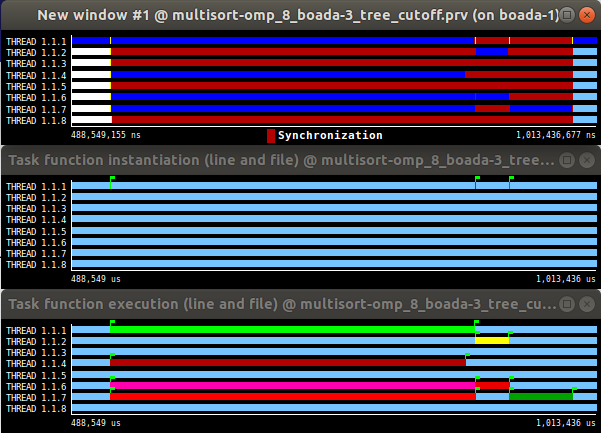
\includegraphics[scale=0.45]{./images/S2/Tree_CUTOFF_paraver}
	
	\label{fig:trace_cutoff_tree}
	\caption{Fragment of the execution flow of the code using the Tree strategy and CUTOFF = 0.}
\end{figure}

As the maximum recursion level is 0, we only create one task for each call function inside multisort. These new tasks will not be able to create tasks, and will execute te code in sequential mode.

In the recursive part, the multisort function does 7 calls (4 for the multisort and 3 for the merge). We can see this 7 created tasks in the third trace in Figure \ref{fig:trace_cutoff_tree}. The four large executions correspond to the multisort functions. Once the first two terminate, the first merge call (yellow one) can be executed. The same happens with the second merge call (red one) when the other two multisort functions end. Finally, the third merge function can start when the other two merge calls have terminated. This happens because of the taskgroup clause.

Once we have understood the cut-off mechanism, we are going to explore the performance of the code when using different values for the maximum recursion level. To do this, we have used the \textbf{submit-cutoff-omp.sh} script.

\begin{figure}[H]
	\centering
	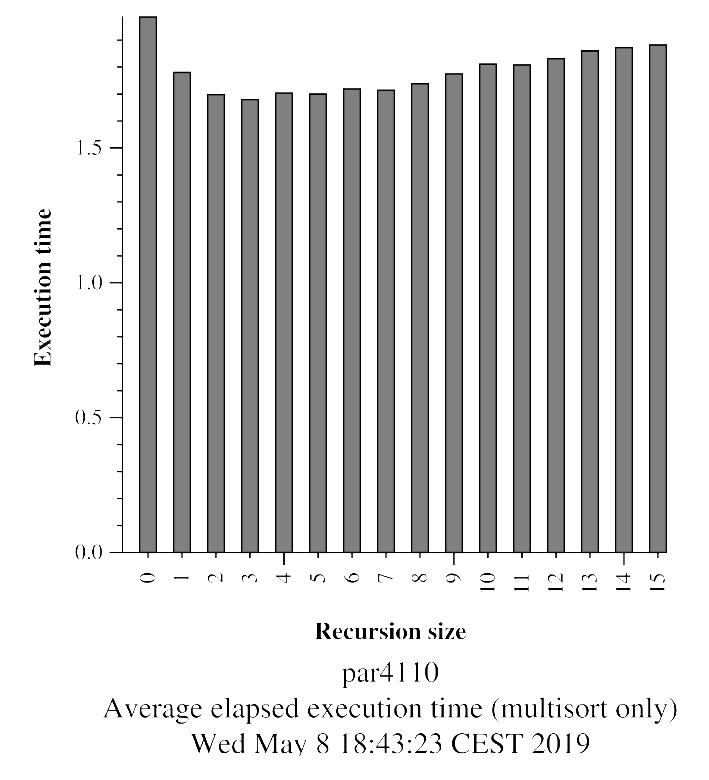
\includegraphics[scale=0.55]{./images/S2/multisort-omp-4-cutoff}
	
	\label{fig:multivalues_cutoff}
	\caption{Execution time of the code when varying the recursion size.}
\end{figure}

With a recursion size value of 3 we get the best performance of the program. Analysing the scalability of the program using this optimum value, we see that the speed-up of the multisort function only is the best in comparison with the other two speed-up plots (Leaf and Tree strategies). However, the difference with the plot of the Tree strategy without the cut-off mechanism is very small.

\begin{figure}[H]
\centering
\begin{minipage}[b]{0.4\linewidth}
  \centering
  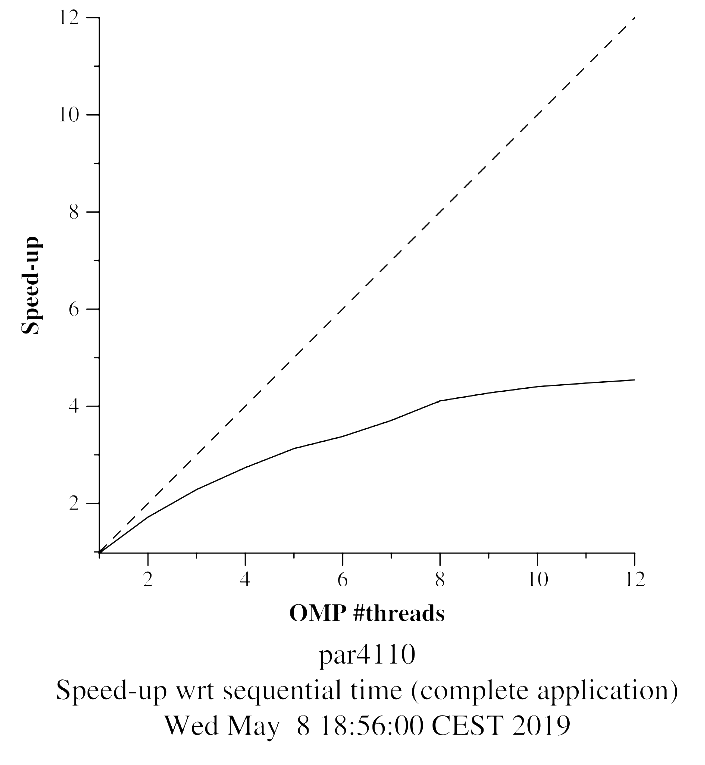
\includegraphics[scale=0.5]{./S2/S2_strong_scalability/multisort-omp-strong_boada-4_tree_cutoff_complete_application}
  \caption{Speed-up plot of the complete application using the Tree strategy and the cut-off mechanism.}
  \label{fig:mandel-omp-10000-strong-21-time}
\end{minipage}%
\hspace{0.5cm}
\begin{minipage}[b]{0.4\linewidth}
  \centering
  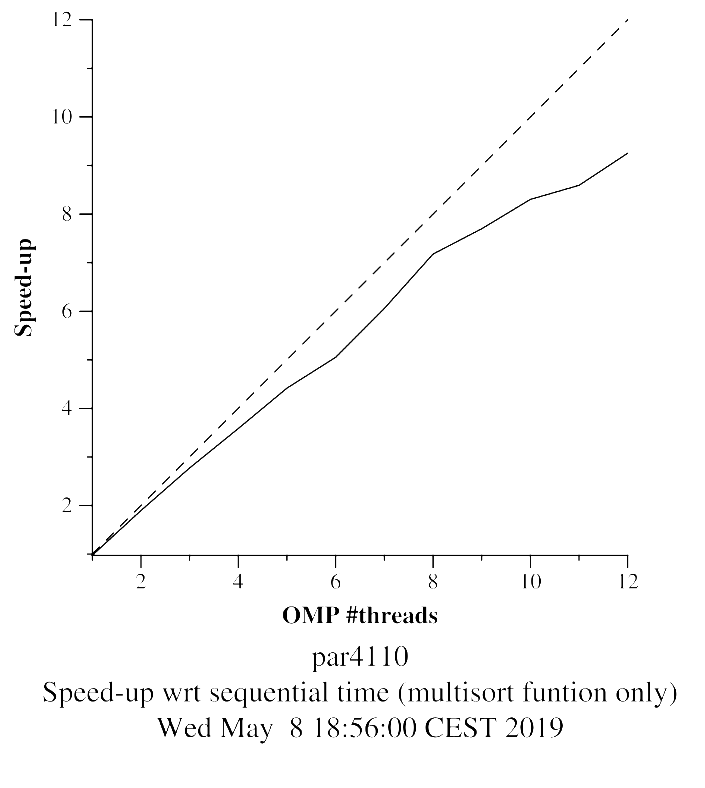
\includegraphics[scale=0.5]{./S2/S2_strong_scalability/multisort-omp-strong_boada-4_tree_cutoff_multisort_only}
  \caption{Speed-up plot of the multisort function using the Tree strategy and the cut-off mechanism.}
  \label{fig:mandel-omp-10000-strong-21-speedup}
\end{minipage}
\end{figure}

\break

\textbf{1. Include the relevant portion of the codes that implement the two versions (Leaf and Tree), commenting whatever necessary.}

\textbf{2. For the the Leaf and Tree strategies, include the speed–up (strong scalability) plots that have been
obtained for the different numbers of processors. Reason about the performance that is observed,
including captures of Paraver windows to justify your explanations.}

\textbf{3. Show the changes you have done in the code in order to include a cut-off mechanism based on
recursion level. Is there a value for the cut-off argument that improves the overall performance?
Analyze the scalability of your parallelization with this value.}

\section{Parallelization and performance analysis with dependent tasks}

In the previous sections we used \textit{\#pragma omp taskwait} and \textit{\#pragma omp taskgroup} to synchronize the tasks. However, it may happen that the execution time of one task is much greater than the other ones. As a result, we will loose time waiting that task to terminate.

A solution to this problem is to get rid of these two \textit{OpenMP} clauses and use the \textit{depend} clause to express dependencies. With this new clause, tasks do not have to wait until all previous tasks end but only the tasks that create their dependencies.

The new code is in \textit{multisort-omp-tree-depend.c} file inside the codes directory.

\begin{figure}[H]
\begin{lstlisting}
void merge(long n, T left[n], T right[n], T result[n*2], long start,
		   long length) {
    if (length < MIN_MERGE_SIZE*2L) {
        // Base case
        basicmerge(n, left, right, result, start, length);
    } else {
        // Recursive decomposition
        #pragma omp task
        merge(n, left, right, result, start, length/2);
        
        #pragma omp task
        merge(n, left, right, result, start + length/2, length/2);
        
        #pragma omp taskwait
    }
}
\end{lstlisting}

\caption{Merge function implementing the Tree strategy using the dependence clauses.}
\end{figure}

\begin{figure}[H]
\begin{lstlisting}
void multisort(long n, T data[n], T tmp[n]) {
    if (n >= MIN_SORT_SIZE*4L) {
        // Recursive decomposition
		#pragma omp task depend(out:data[0])
		multisort(n/4L, &data[0], &tmp[0]);
		
		#pragma omp task depend(out:data[n/4L])
		multisort(n/4L, &data[n/4L], &tmp[n/4L]);
		
		#pragma omp task depend(out:data[n/2L])
		multisort(n/4L, &data[n/2L], &tmp[n/2L]);
		
		#pragma omp task depend(out:data[3L*n/4L])
		multisort(n/4L, &data[3L*n/4L], &tmp[3L*n/4L]);

		
		#pragma omp task depend(in:data[0],data[n/4L]) 
						 depend(out:tmp[0])
		merge(n/4L, &data[0], &data[n/4L], &tmp[0], 0, n/2L);
		
		#pragma omp task depend(in:data[n/2L],data[3L*n/4L])
						 depend(out:tmp[n/2L])
		merge(n/4L, &data[n/2L], &data[3L*n/4L], &tmp[n/2L], 0, n/2L);
		
		#pragma omp task depend(in:tmp[0],tmp[n/2L])
        merge(n/2L, &tmp[0], &tmp[n/2L], &data[0], 0, n);
        
        #pragma omp taskwait
	} else {
		// Base case
		basicsort(n, data);
	}
}
\end{lstlisting}

\caption{Multisort function implementing the Tree strategy using the dependence clauses.}
\end{figure}

The first merge call cannot be executed until the previous tasks with \textit{depend(out: data[0])} and \textit{depend(out: data[n/4L])} terminate. Now, even though the third or fourth multisort calls have not terminated, the first merge call can be executed. The same happens for the rest of the calls with the depend clause. Thus, we will reduce a bit the execution time of the program.

Nevertheless, we must use \textit{\#pragma omp taskwait} at the end of both multisort and merge functions. Without them, the sorting would not be correct because it could happen that while the last merge call inside the multisort function is being executed, we terminate this function and start with other tasks. The next task would think that the vector is already sorted altough that merge call would have not terminated yet. The same happens inside the merge function.

The most important thing we see in Figure \ref{fig:depend_tree} is that there is even less parts in Idle time than in the Tree flow (Figure \ref{fig:tree_traces}). Hence, the execution time is reduced a bit with respect to the one using the Tree strategy.

\begin{figure}[H]
	\centering
	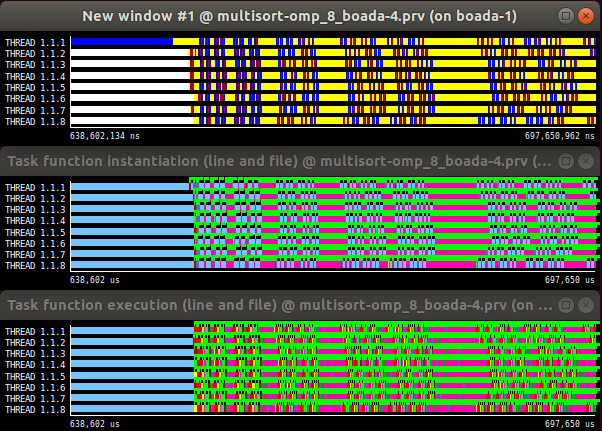
\includegraphics[scale=0.45]{./images/S3/Tree_depend_paraver}

	\label{fig:depend_tree}	
	\caption{Fragment of the execution flow of the code using the Tree strategy and the depend clause.}
\end{figure}

Finally, in the scalability plots of this program we can observe that both have the best speed-ups with respect to all previous speed-up plots. This has been possible with the use of the depend clause.

\begin{figure}[H]
\centering
\begin{minipage}[b]{0.4\linewidth}
  \centering
  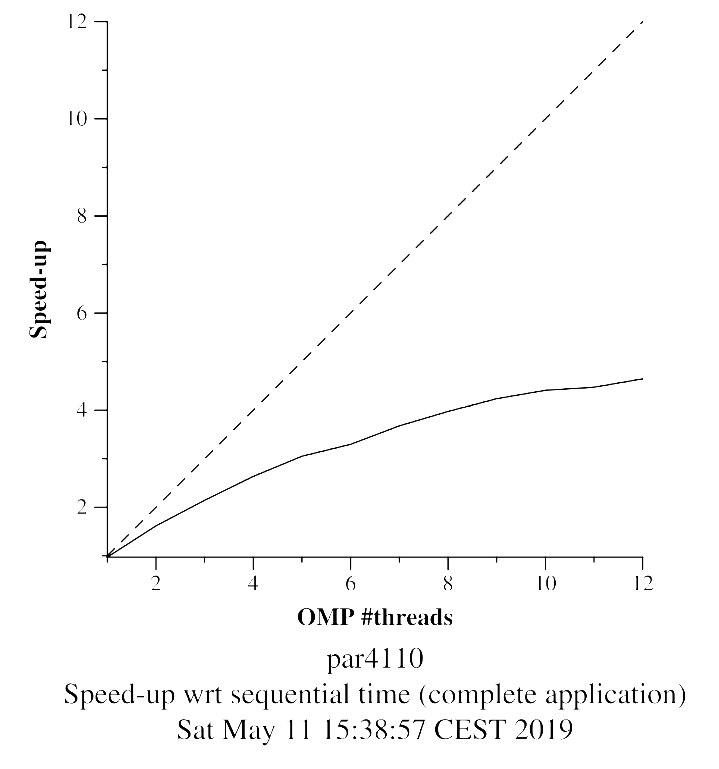
\includegraphics[scale=0.5]{./images/S3/multisort-omp-strong_boada-2_tree_depend_complete_application}
  \caption{Speed-up plot of the complete application using the Tree strategy and the cut-off mechanism.}
  \label{fig:mandel-omp-10000-strong-21-time}
\end{minipage}%
\hspace{0.5cm}
\begin{minipage}[b]{0.4\linewidth}
  \centering
  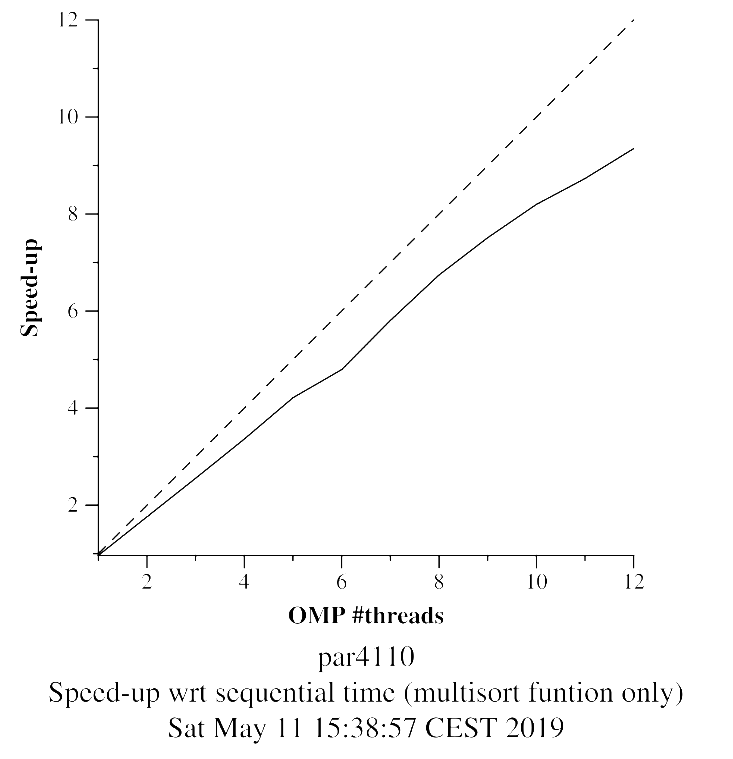
\includegraphics[scale=0.5]{./images/S3/multisort-omp-strong_boada-2_tree_depend_multisort_only}
  \caption{Speed-up plot of the multisort function using the Tree strategy and the cut-off mechanism.}
  \label{fig:mandel-omp-10000-strong-21-speedup}
\end{minipage}
\end{figure}

\break

\textbf{1. Include the relevant portion of the code that implements the Tree version with task dependencies,
commenting whatever necessary.}

\textbf{2. Reason about the performance that is observed, including the speed–up plots that have been
obtained for different numbers of processors and with captures of Paraver windows to justify your
reasoning.}

\section{Optional}

\subsection{Optional 1}

In this part we used the code from the section \nameref{treestrategy}, to check the different resources of each Boada node.

\subsubsection{Boada-1 to 4}

As we have seen in the First Laboratory, the number of cores of these nodes is 12. Executing the script in one of those nodes we obtained the following Speed-up plots.

\begin{figure}[H]
\centering
\begin{minipage}[b]{0.4\linewidth}
  \centering
  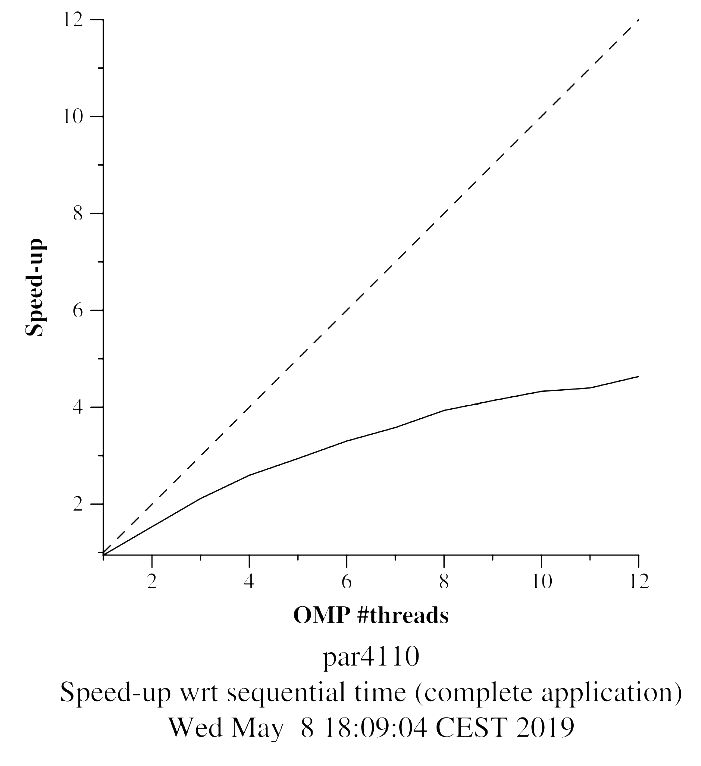
\includegraphics[scale=0.5]{./S2/S2_strong_scalability/multisort-omp-strong_boada-3_tree_complete_application}
  \caption{Speed-up plot of the complete application using the Tree strategy in Boada 3.}
  \label{fig:mandel-omp-10000-strong-21-time}
\end{minipage}%
\hspace{0.5cm}
\begin{minipage}[b]{0.4\linewidth}
  \centering
  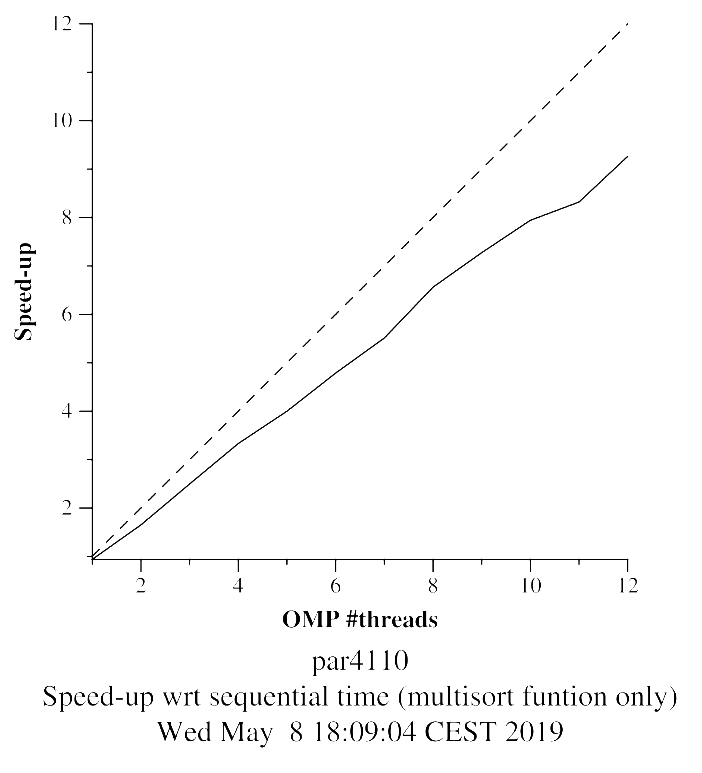
\includegraphics[scale=0.5]{./S2/S2_strong_scalability/multisort-omp-strong_boada-3_tree_multisort_only}
  \caption{Speed-up plot of the multisort function using the Tree strategy in Boada 3.}
  \label{fig:mandel-omp-10000-strong-21-speedup}
\end{minipage}
\end{figure}

\subsubsection{Boada-5}

In this node we have a total of 12 cores, equal that in Boada-1 to 4, but in this node we have a different architecture. Submitting with the script we obtained the following results.

\begin{figure}[H]
\centering
\begin{minipage}[b]{0.4\linewidth}
  \centering
  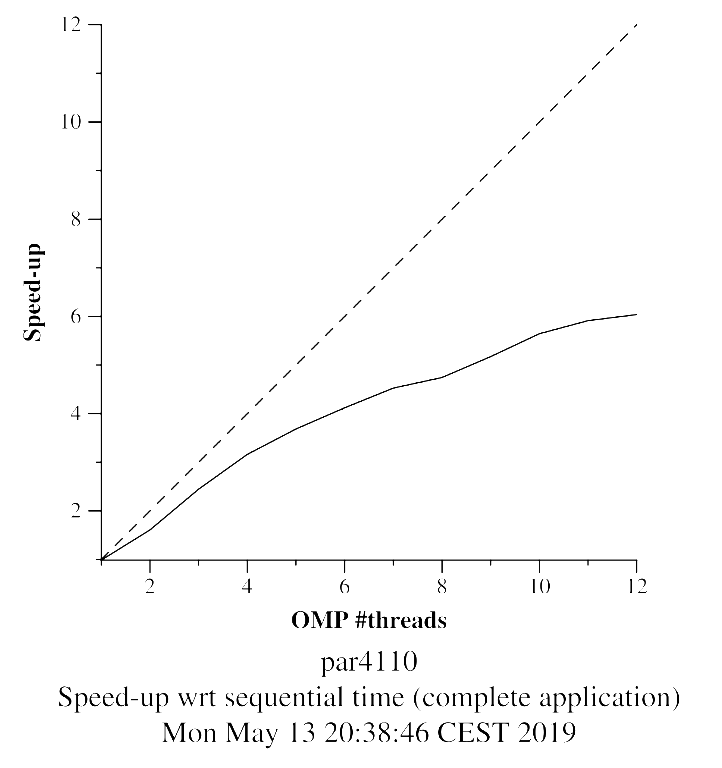
\includegraphics[scale=0.5]{./S2/multisort-omp-strong_boada-5_tree_complete_application}
  \caption{Speed-up plot of the complete application using the Tree strategy in Boada 5.}
  \label{fig:mandel-omp-10000-strong-21-time}
\end{minipage}%
\hspace{0.5cm}
\begin{minipage}[b]{0.4\linewidth}
  \centering
  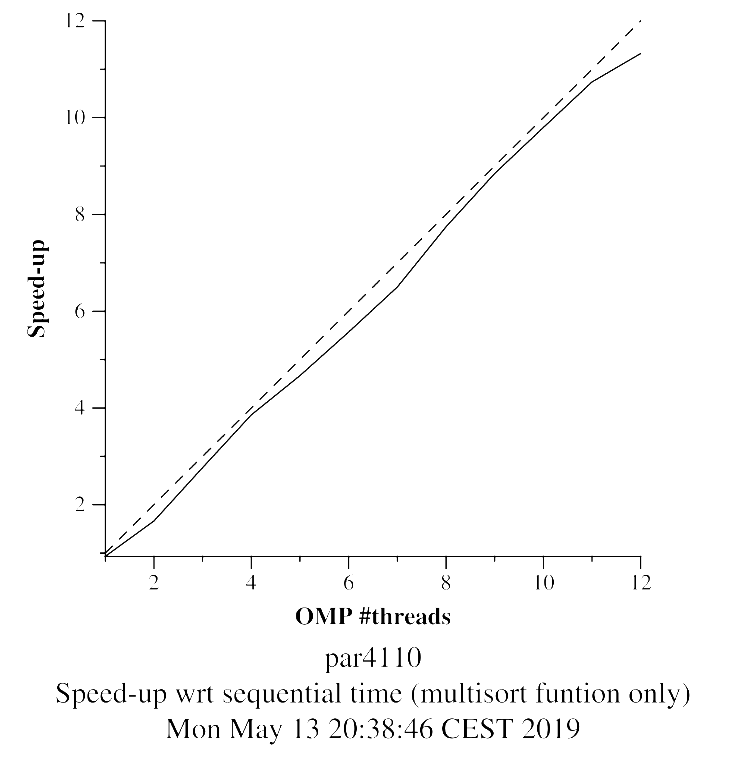
\includegraphics[scale=0.5]{./S2/multisort-omp-strong_boada-5_tree_multisort_only}
  \caption{Speed-up plot of the multisort function using the Tree strategy in Boada 5.}
  \label{fig:mandel-omp-10000-strong-21-speedup}
\end{minipage}
\end{figure}

\subsubsection{Boada-6 to 8}

In this case, these nodes have a total of 16 cores. So we have changed the value of np_NMAX to 16 in the submit-strong-omp.sh script. Afterwards we executed the script in one of these nodes.

\begin{figure}[H]
\centering
\begin{minipage}[b]{0.4\linewidth}
  \centering
  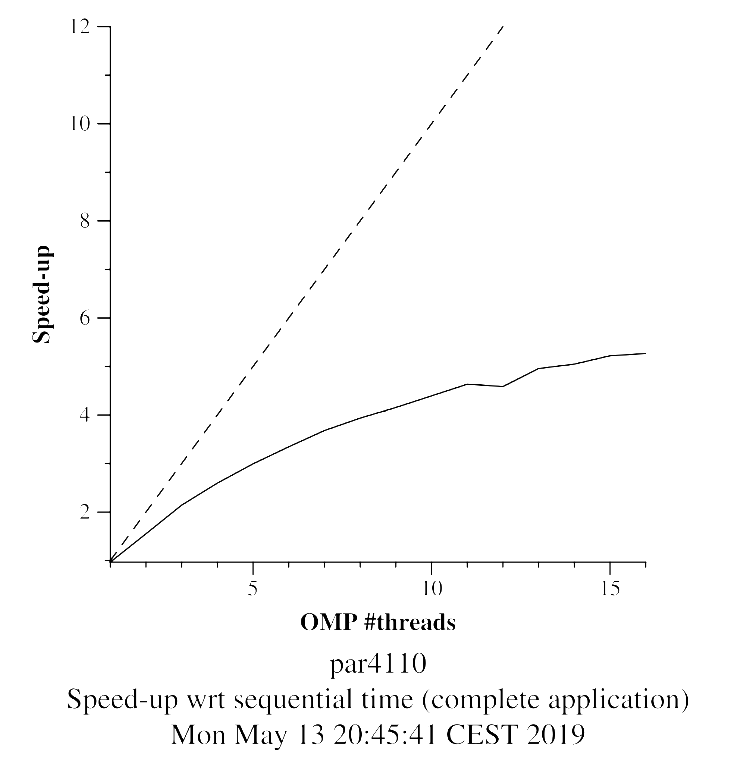
\includegraphics[scale=0.5]{./S2/multisort-omp-strong_boada-7_tree_complete_application}
  \caption{Speed-up plot of the complete application using the Tree strategy in Boada 7.}
  \label{fig:mandel-omp-10000-strong-21-time}
\end{minipage}%
\hspace{0.5cm}
\begin{minipage}[b]{0.4\linewidth}
  \centering
  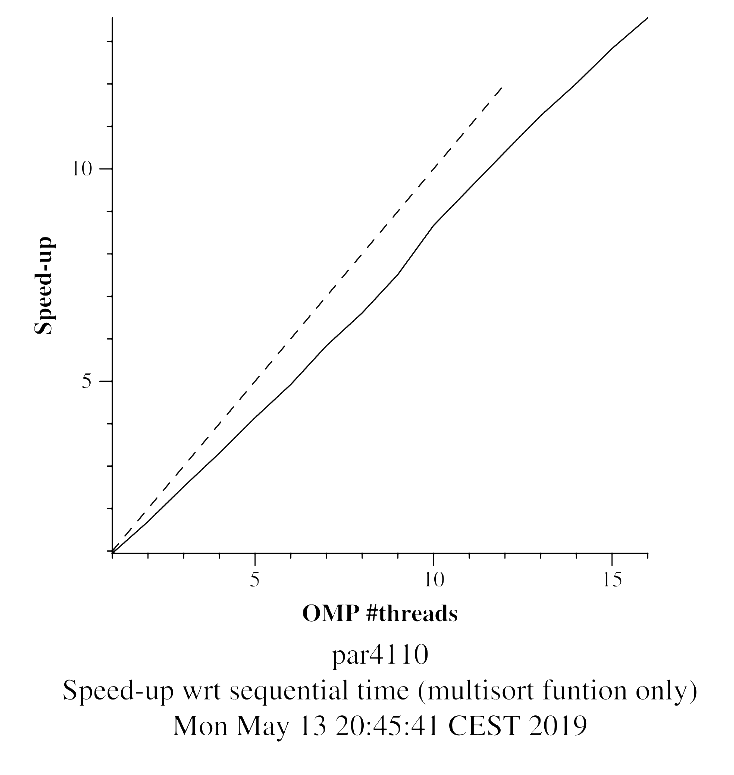
\includegraphics[scale=0.5]{./S2/multisort-omp-strong_boada-7_tree_multisort_only}
  \caption{Speed-up plot of the multisort function using the Tree strategy in Boada 7.}
  \label{fig:mandel-omp-10000-strong-21-speedup}
\end{minipage}
\end{figure}

We have seen that the beest resultss are in the Boada-5, due to the architecture of this node, which has the best maximum core frequency.

\section{Annex}

\subsection{Scalability anaysis: Traces using different number of processors}

\begin{figure}[H]
	\centering
	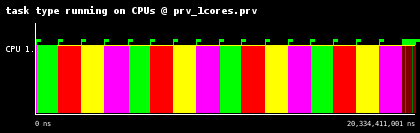
\includegraphics[scale=0.75]{./images/S1_scalability/S1_scalability_1}
	
	\label{fig_ann:S1_scalability_1}
	\caption{Execution flow of the code using 1 processor.}
\end{figure}





\begin{figure}[H]
	\centering
	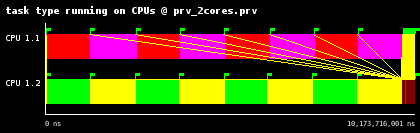
\includegraphics[scale=0.75]{./images/S1_scalability/S1_scalability_2}
	
	\label{fig_ann:S1_scalability_2}
	\caption{Execution flow of the code using 2 processors.}
\end{figure}





\begin{figure}[H]
	\centering
	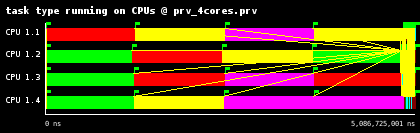
\includegraphics[scale=0.75]{./images/S1_scalability/S1_scalability_4}
	
	\label{fig_ann:S1_scalability_4}
	\caption{Execution flow of the code using 4 processors.}
\end{figure}





\begin{figure}[H]
	\centering
	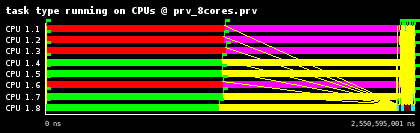
\includegraphics[scale=0.75]{./images/S1_scalability/S1_scalability_8}
	
	\label{fig_ann:S1_scalability_8}
	\caption{Execution flow of the code using 8 processors.}
\end{figure}





\begin{figure}[H]
	\centering
	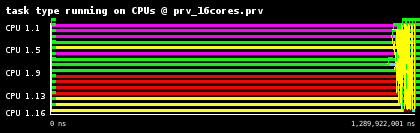
\includegraphics[scale=0.75]{./images/S1_scalability/S1_scalability_16}
	
	\label{fig_ann:S1_scalability_16}
	\caption{Execution flow of the code using 16 processors.}
\end{figure}





\begin{figure}[H]
	\centering
	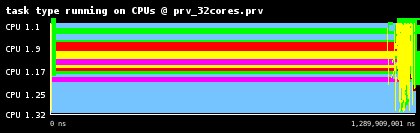
\includegraphics[scale=0.75]{./images/S1_scalability/S1_scalability_32}
	
	\label{fig_ann:S1_scalability_32}
	\caption{Execution flow of the code using 32 processors.}
\end{figure}





\begin{figure}[H]
	\centering
	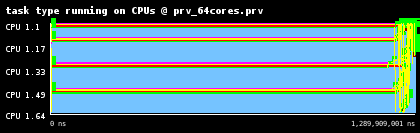
\includegraphics[scale=0.75]{./images/S1_scalability/S1_scalability_64}
	
	\label{fig_ann:S1_scalability_64}
	\caption{Execution flow of the code using 64 processors.}
\end{figure}

\end{document} 